\section{Introduction}

It has been estimated that 50 million dengue cases infect people per year and there are approximately 2.5 billion people living in dengue-prone areas (tropics and urban settings). The number of dengue cases have been higher than ever. In 1955-1959 only 908 cases of dengue were recorded. A very steep rise in just a span of 60 years\cite{who:dengue}. This is mostly caused by the rise in population and having more dense urban living space.

The main vector for the dengue virus, mosquito \textit{Aedes Aegypti}, has adapted to the conditions of urban areas in humid and temperate countries \cite{descloux,carlos}. In locations where clear water is abundant and its temperature is just right, the female Aedes lays her eggs. Studying the vectors in this certain environment can be helpful in the planning and mapping of the locations of prime breeding locations and "hotspots" for female Aedes\cite{who:dengue}. Having this ability means being able to control Aedes population.

Models which utilize spatial aspects and also include time in their construction makes control more efficient. \textbf{MOMA} (Model Of Mosquito Aedes) is a model developed with space and time in mind and also utilizes the geographical outline and formation of a certain neighbourhood. This model uses Geographical Information Systems and Agent-Based Models for mapping the objects in this environment and the latter for giving the Aedes mosquito detailed behaviour

\section{Background}



\subsection{Previous Models}

\textbf{MOMA} is a behavioural model that surveys a large area representing a neighbourhood. It takes into account breeding sites\cite{skeeter,carlos}, human density, topology and this sets it apart from previous models.

\subsubsection{Skeeter-Buster} 

Skeeter-Buster's main focus is on breeding site dynamics \cite{skeeter}. It is a stochastic, spatially-explicit model that models cohorts of mosquitoes at a very fine spatial scale, down to the level of individual breeding sites for immature cohorts, or individual houses for adults. Skeeter Buster additionally includes a detailed genetic component, and can therefore model the genetics of Ae. aegypti populations, making it a crucial tool in the evaluation and development of genetic control strategies. 

The main difference of it from MOMA is that Skeeter-Buster does not incorporate blood stocks from humans. It also differs from MOMA because of its scale. Skeeter-Buster focuses on the contents of individual houses and the individual water-containers where the Aedes lays their egg and where their eggs develop into other vectors. 

\subsubsection{SimPopMosq}

This model is the considered closest to the MOMA. It includes the blood stock in the model for the mosquitoes. This model allows for interactions between the mosquito and people but only in a very small vicinity\cite{sandro}. It adds a spatial aspect to the frequently used CIMSiM model. 

The CIMSiM Model estimates the capacity of the production of mosquito larvae in a vector site under varying temperatures and humidity or precipitation. This approach was also utilized and adapted by Skeeter Buster to model intra-container development.

The SimPopMosq model is based on the interaction of agent-based model made up of four classes (Aedes,human,dog and cat) with environmental data (vector,bedroom and garden). This model is used to study the dispersal and movement of Aedes indoors and gardens, and also studies the effeciency of mosquito trap placements.


\subsection{Assumptions}
The breeding site dynamics are mainly affected by temperature, precipitation and the land-use categories of the location generated by the Geographical Information System. It can speed up, slow down or kill Aedes offsprings. We can also assume that the urban space and topology will affect the population dynamics of our dengue vector. As these items locate where possible breeding sites of the Aedes will be, locations of the blood stocks (humans) and areas with shade is also defined by the urban topology of the desired location.

\section{Methods}

The model was created using Gama 1.6.1. This software gives the ability to use graphical modelling tools and manipulation of the GIS data. Being able to manipulate the GIS data in this software is the main reason this tool was used. Other softwares used in this study are QGIS (2.6.1) and R (x64 3.2.0). QGIS was used for obtaining the environmental data of the model and R was used for analysis of simulation results.


\subsection{Significance of model}
This model's main purpose is that it models and watches Aedes population dynamics in an urban setting having a dense and cramped setting. The main agent observed in this model is the agent Aedes, this agent is our main vector for the dengue virus. This agent is able to bite, mate, rest, oviposit, and interact with objects that consume space. 

The setting of this model is affected by the real-world meteorogical data and the daily temperature of the desired location to simulate. In this study a neighbourhood in Delhi, India; was simulated. In this setting, precipitation is high and temperature for breeding sites is near or is ideal, since this India has a tropic climate.

\subsection{Entities, State variables and Scales}

The model has two categories of agents in the model (1) mobile agents called Aedes representing female Ae. Aegypti and (2) spatial objects called SpatObj that correspond to the physical environment. 

An overall environment for the simulation that contains simulation parameters and meteorogical data, and acts as a daily Aedes killer in accordance to nominal daily survival probability assigned for each day \cite{magori}  from Skeeter Buster called World.

Only female adult Ae. Aegypti mosquito called \textbf{Aedes} was represented because males do not transmit dengue while mating is simulated by applying mating probability. 

Each Aedes has the following state variables:

\begin{itemize}
    \item \textbf{Age}: The age of Aedes determines whether the Aedes should be kept or removed in the model through its Age limit and from the first day of emergence, starting from day 0. The age limit is determined during instantiation according to a distribution law.
    \item \textbf{Stage}: Aedes was assumed to have four stages in its life: \textit{virgin} for a non-inseminated mosquito, \textit{ovipo} for a mated female which has not taken a meal yet, \textit{gono} for one which already taken a blood meal and started its gonotrophic cycle (waiting to lay eggs), and death which will remove it from simulation. When a \textit{gono} female lays its eggs, it becomes once again a \textit{ovipo} female till its next blood meal(s). Each stage has different behavior that leads to specific activities (bite, fly, lay egg, and rest).
    \item \textbf{Best Target}: The best target represents what the Aedes needs at the time it usually needs a breeding site, a blood meal, nectar or shade. The need of the Aedes is determined according to the stage of the Aedes, quantity of blood stock, energy level and availability of the targets in the mosquito's perception. 
    \item \textbf{Quantity of blood stock}: The quantity of blood stock is used as an indicator to start the gonotrophic cycle it also influences the target selection process.
    \item \textbf{Energy Level}: The energy level varies depending on what current activity the Aedes is doing, it also influences the target selection process.
    \item \textbf{Current Location}: Aedes is a mobile agent. The current location is where the Aedes currently is, the location is indicated through coordinates (x,y) in the World .
    \item \textbf{Current Activity}: The current activity at time t. The activities are (a) biting, (b) taking nectar, (c) laying eggs and (d) resting.
\end{itemize}

\begin{figure*}
  \centering 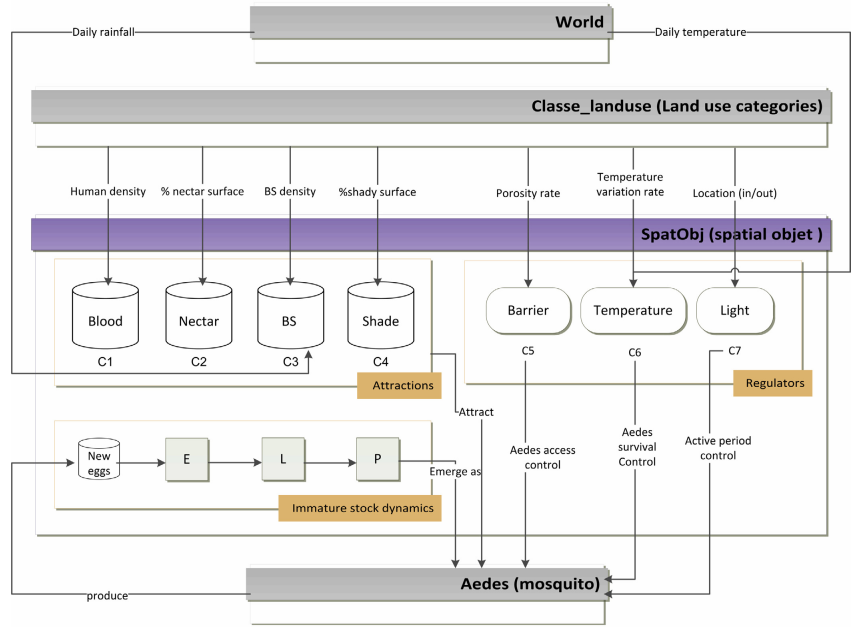
\includegraphics[width = 17cm]{fig1.PNG}
  \caption{The Organization level of information flux participating in the dynamics of SpatObj which has an impact on Aedes life cycle.}
\end{figure*}

These state variables describe the mathematical state of the model which helps to determine its future behavior in the absence of any external forces affecting the system. Also, it gives a description of the the SpatObj form the point of view of the Ae. Agypti's needs and constraints

SpatObj is where an Aedes can locate itself and with which it can interact. This is environment is defined as a resource-based habitat for the mosquito. The Resources are needed to meet the Aedes' goals (bite, rest, oviposit, etc.) are available through input description of the environmental shape file process with Geographic Information System (GIS).

A SpatObj agent contains four targets that attract a mosquito,
\begin{itemize}
    \item Blood (C1)
    \item Nectar (C2)
    \item Breeding site (C3)
    \item Shade (C4)
\end{itemize}
four stocks of immature Aedes,
\begin{itemize}
    \item new eggs
    \item eggs (submerged)
    \item larvae
    \item pupae
\end{itemize}
and three characteristics that regulate Aedes' activities,
\begin{itemize}
    \item Porosity (C5) which affects the mosquito movement
    \item temperature (C6) for survival rate
    \item light level (C7) for active period. 
\end{itemize}


Variations of these attributes can be dynamic because of the space characterized environmental heterogeneity.

Interaction between an Aedes and its environmental can occur only via SpatObj. Which means even though temperature and rainfall are global variables of the world the are only accessible through SpatObj. Each SpatObj takes, as an input, an overall value and computes a new value of these factors depending on its own parameters.

All these agents can be organized to produce a macroscopic scale (World) through mesoscopic scale (SpatObj) to a microscopic scale (Aedes). Figure 1 presents this organization and the links between input data and the SpatObj's resource available for Aedes.



\subsection{Process overview and Scheduling}

A mosquito spends some activities that last a few seconds whereas others can take hours. The model's time step is fixed at one minute which was determined according to the shortest event we expect to study in future scenarios, that is, the biting activity, with the constraint that the model must be run over a period of several months.

Various time frames linked to specific processes are present in a simulation:

\begin{enumerate}
      \item \textbf{Every day}, the SpatObj agents uses the information stocked in the agent World to define the local air and water temperature also each day, the Aedes grow old by 1.
      \item \textbf{Every hour}, the SpatObj agents update their lighting which controls the activity period, and blood resource levels which depends on the availability of human beings. 
      \item \textbf{Every second}, the Aedes agent select the best target. If they have at least one need, the Aedes will behave according to the \textbf{ Behavior decision-making process}. If none can satisfy the need of the Aedes, it will move randomly. Otherwise, it will move towards the target according to the procedure \textbf{movement and dispersal}.
\end{enumerate}
  


\appendix
%Appendix A
\section{Headings in Appendices}
The rules about hierarchical headings discussed above for
the body of the article are different in the appendices.
In the \textbf{appendix} environment, the command
\textbf{section} is used to
indicate the start of each Appendix, with alphabetic order
designation (i.e., the first is A, the second B, etc.) and
a title (if you include one).  So, if you need
hierarchical structure
\textit{within} an Appendix, start with \textbf{subsection} as the
highest level. Here is an outline of the body of this
document in Appendix-appropriate form:
\subsection{Introduction}
\subsection{The Body of the Paper}
\subsubsection{Type Changes and  Special Characters}
\subsubsection{Math Equations}
\paragraph{Inline (In-text) Equations}
\paragraph{Display Equations}
\subsubsection{Citations}
\subsubsection{Tables}
\subsubsection{Figures}
\subsubsection{Theorem-like Constructs}
\subsubsection*{A Caveat for the \TeX\ Expert}
\subsection{Conclusions}
\subsection{References}
\bibliographystyle{ACM-Reference-Format}
\bibliography{bibliography}
% This next section command marks the start of
% Appendix B, and does not continue the present hierarchy
\section{More Help for the Hardy}

Of course, reading the source code is always useful.  The file
\path{acmart.pdf} contains both the user guide and the commented
code.

\begin{acks}
  Acknowledgments here...

\end{acks}
%\end{document}  % This is where a 'short' article might terminate